\documentclass[a4paper]{article}
\renewcommand{\epsilon}{\varepsilon}
\newcommand{\triposcourse}{Numerical Analysis}
\usepackage{fancyhdr,titlesec,geometry}
\usepackage[dvipsnames]{xcolor}
\usepackage[many]{tcolorbox}
\usepackage{xifthen}
\usepackage{import}
\usepackage{parskip}
\usepackage{transparent}
\usepackage{mathtools,amssymb,amsfonts,amsthm,bm}   % Math Presets
\usepackage{array,tabularx,booktabs}                % Table Presets
\usepackage{graphicx,wrapfig,float,caption}         % Figure Presets
\usepackage{setspace,multicol}                      % Text Presets
\usepackage{tikz,physics,cancel,tkz-euclide,pgfplots,tikz-3dplot}                    % Physics Presets
\usepackage{amsmath}
\usepackage{mathrsfs}
\usepackage{enumerate}
\usepackage[shortlabels]{enumitem}
\usepackage{hyperref}
\usepackage{lipsum}
\usepackage{IEEEtrantools}
\usepackage{xcomment}
\usepackage{sectsty}
\usepackage{thmtools}
\usepackage{mdframed}
\usepackage{siunitx}
\usepackage{centernot}

\newcommand{\sectionbreak}{\clearpage}

\tdplotsetmaincoords{60}{120}

\usetikzlibrary{arrows.meta}
\usetikzlibrary{decorations.markings}
\usetikzlibrary{decorations.pathmorphing}
\usetikzlibrary{automata, positioning}
\usetikzlibrary{fadings}
\usetikzlibrary{intersections}
\usetikzlibrary{cd}
\usetikzlibrary{patterns}
\usetikzlibrary{shapes.arrows}
\usepgfplotslibrary{colormaps, external}
\pgfarrowsdeclarecombine{twolatex'}{twolatex'}{latex'}{latex'}{latex'}{latex'}
\tikzset{->/.style = {decoration={markings,
                                  mark=at position 1 with {\arrow[scale=1.6]{latex'}}},
                      postaction={decorate}}}
\tikzset{<-/.style = {decoration={markings,
                                  mark=at position 0 with {\arrowreversed[scale=1.6]{latex'}}},
                      postaction={decorate}}}
\tikzset{<->/.style = {decoration={markings,
                                   mark=at position 0 with {\arrowreversed[scale=1.6]{latex'}},
                                   mark=at position 1 with {\arrow[scale=1.6]{latex'}}},
                       postaction={decorate}}}
\tikzset{->-/.style = {decoration={markings,
                                   mark=at position #1 with {\arrow[scale=1.6]{latex'}}},
                       postaction={decorate}}}
\tikzset{-<-/.style = {decoration={markings,
                                   mark=at position #1 with {\arrowreversed[scale=1.6]{latex'}}},
                       postaction={decorate}}}
\tikzset{->>/.style = {decoration={markings,
                                  mark=at position 1 with {\arrow[scale=1.6]{twolatex'}}},
                      postaction={decorate}}}
\tikzset{<<-/.style = {decoration={markings,
                                  mark=at position 0 with {\arrowreversed[scale=1.6]{twolatex'}}},
                      postaction={decorate}}}
\tikzset{<<->>/.style = {decoration={markings,
                                   mark=at position 0 with {\arrowreversed[scale=1.6]{twolatex'}},
                                   mark=at position 1 with {\arrow[scale=1.6]{twolatex'}}},
                       postaction={decorate}}}
\tikzset{->>-/.style = {decoration={markings,
                                   mark=at position #1 with {\arrow[scale=1.6]{twolatex'}}},
                       postaction={decorate}}}
\tikzset{-<<-/.style = {decoration={markings,
                                   mark=at position #1 with {\arrowreversed[scale=1.6]{twolatex'}}},
                       postaction={decorate}}}

\tikzset{
set arrow inside/.code={\pgfqkeys{/tikz/arrow inside}{#1}},
set arrow inside={end/.initial=>, opt/.initial=},
/pgf/decoration/Mark/.style={
    mark/.expanded=at position #1 with
    {
        \noexpand\arrow[\pgfkeysvalueof{/tikz/arrow inside/opt}]{\pgfkeysvalueof{/tikz/arrow inside/end}}
    }
},
arrow inside/.style 2 args={
    set arrow inside={#1},
    postaction={
        decorate,decoration={
            markings,Mark/.list={#2}
        }
    }
},
}

\tikzstyle{circ}=[fill=black, draw=black, shape=circle]
\tikzset{
dot/.style = {circle, fill, minimum size=#1,
              inner sep=0pt, outer sep=0pt},
dot/.default = 5pt% size of the circle diameter 
}
\tikzset{mstate/.style={circle, draw, blue, text=black, minimum width=0.7cm}}
\tikzset{snake it/.style={-stealth,
decoration={snake, 
    amplitude = .4mm,
    segment length = 2mm,
    post length=0.9mm},decorate}}

\def\centerarc[#1](#2)(#3:#4:#5)% Syntax: [draw options](center)(initial angle:final angle:radius)
    { \draw[#1] ($(#2)+({#5*cos(#3)},{#5*sin(#3)})$) arc (#3:#4:#5); }

\hypersetup{
    colorlinks=true,
    linkcolor=blue,
    filecolor=blue,
    citecolor = black,      
    urlcolor=cyan,
    }

%%%%%%%%%%% Snippets %%%%%%%%%%%%%%%%
\newcommand*\widefbox[1]{\fbox{\hspace{2em}#1\hspace{2em}}}
\newcommand{\xint}{\int_{x_1}^{x_2}}
\newcommand{\mw}{\sqrt{m\omega}}
\newcommand{\de}{\delta}
\newcommand{\dde}{\dot{\delta}}
\newcommand{\di}{\delta_i}
\newcommand{\ddi}{\dot{\delta_i}}
\newcommand{\dddi}{\ddot{\delta_i}}
\newcommand{\dipl}{\delta_{i+1}}
\newcommand{\dimi}{\delta_{i-1}}
\newcommand{\ddt}[1]{\frac{{d} #1}{dt}}
\newcommand{\ddtt}[1]{\frac{d^2 #1}{dt^2}}
\newcommand{\ddx}[1]{\frac{d #1}{dx}}
\newcommand{\ddxx}[1]{\frac{d^2 #1}{dx^2}}
\newcommand{\eps}{\epsilon}
\newcommand{\del}[2]{\frac{\partial #1}{\partial #2}}
\newcommand{\deltwo}[2]{\frac{\partial^2 #1}{\partial #2^2}}
\newcommand{\lam}{\lambda}
\newcommand{\Lam}{\Lambda}
\newcommand{\sig}{\sigma}
\newcommand{\Sig}{\Sigma}
\newcommand{\half}{\frac{1}{2}}
\newcommand{\munu}{{\mu\nu}}
\newcommand{\thalf}{\tfrac{1}{2}}
\renewcommand{\div}{\nabla\cdot}
\renewcommand{\curl}{\nabla\times}

\DeclareMathOperator{\orb}{Orb}
\DeclareMathOperator{\stab}{Stab}
\DeclareMathOperator{\adj}{adj}
\DeclareMathOperator{\ccl}{ccl}
\let\var\relax
\DeclareMathOperator{\var}{Var}
\DeclareMathOperator{\cov}{Cov}
\DeclareMathOperator{\corr}{Corr}
\DeclareMathOperator{\Markov}{Markov}
\DeclareMathOperator{\nullity}{nullity}

\newcommand{\bfA}{{\bf A}}
\newcommand{\bfB}{{\bf B}}
\newcommand{\bfC}{{\bf C}}
\newcommand{\bfD}{{\bf D}}
\newcommand{\bfE}{{\bf E}}
\newcommand{\bfF}{{\bf F}}
\newcommand{\bfG}{{\bf G}}
\newcommand{\bfH}{{\bf H}}
\newcommand{\bfI}{{\bf I}}
\newcommand{\bfJ}{{\bf J}}
\newcommand{\bfK}{{\bf K}}
\newcommand{\bfL}{{\bf L}}
\newcommand{\bfM}{{\bf M}}
\newcommand{\bfN}{{\bf N}}
\newcommand{\bfO}{{\bf O}}
\newcommand{\bfP}{{\bf P}}
\newcommand{\bfQ}{{\bf Q}}
\newcommand{\bfR}{{\bf R}}
\newcommand{\bfS}{{\bf S}}
\newcommand{\bfT}{{\bf T}}
\newcommand{\bfU}{{\bf U}}
\newcommand{\bfV}{{\bf V}}
\newcommand{\bfW}{{\bf W}}
\newcommand{\bfX}{{\bf X}}
\newcommand{\bfY}{{\bf Y}}
\newcommand{\bfZ}{{\bf Z}}

\newcommand{\bfa}{{\bf a}}
\newcommand{\bfb}{{\bf b}}
\newcommand{\bfc}{{\bf c}}
\newcommand{\bfd}{{\bf d}}
\newcommand{\bfe}{{\bf e}}
\newcommand{\bff}{{\bf f}}
\newcommand{\bfg}{{\bf g}}
\newcommand{\bfh}{{\bf h}}
\newcommand{\bfi}{{\bf i}}
\newcommand{\bfj}{{\bf j}}
\newcommand{\bfk}{{\bf k}}
\newcommand{\bfl}{{\bf l}}
\newcommand{\bfm}{{\bf m}}
\newcommand{\bfn}{{\bf n}}
\newcommand{\bfo}{{\bf o}}
\newcommand{\bfp}{{\bf p}}
\newcommand{\bfq}{{\bf q}}
\newcommand{\bfr}{{\bf r}}
\newcommand{\bfs}{{\bf s}}
\newcommand{\bft}{{\bf t}}
\newcommand{\bfu}{{\bf u}}
\newcommand{\bfv}{{\bf v}}
\newcommand{\bfw}{{\bf w}}
\newcommand{\bfx}{{\bf x}}
\newcommand{\bfy}{{\bf y}}
\newcommand{\bfz}{{\bf z}}

\newcommand{\mcA}{{\mathcal{A}}}
\newcommand{\mcB}{{\mathcal{B}}}
\newcommand{\mcC}{{\mathcal{C}}}
\newcommand{\mcD}{{\mathcal{D}}}
\newcommand{\mcE}{{\mathcal{E}}}
\newcommand{\mcF}{{\mathcal{F}}}
\newcommand{\mcG}{{\mathcal{G}}}
\newcommand{\mcH}{{\mathcal{H}}}
\newcommand{\mcI}{{\mathcal{I}}}
\newcommand{\mcJ}{{\mathcal{J}}}
\newcommand{\mcK}{{\mathcal{K}}}
\newcommand{\mcL}{{\mathcal{L}}}
\newcommand{\mcM}{{\mathcal{M}}}
\newcommand{\mcN}{{\mathcal{N}}}
\newcommand{\mcO}{{\mathcal{O}}}
\newcommand{\mcP}{{\mathcal{P}}}
\newcommand{\mcQ}{{\mathcal{Q}}}
\newcommand{\mcR}{{\mathcal{R}}}
\newcommand{\mcS}{{\mathcal{S}}}
\newcommand{\mcT}{{\mathcal{T}}}
\newcommand{\mcU}{{\mathcal{U}}}
\newcommand{\mcV}{{\mathcal{V}}}
\newcommand{\mcW}{{\mathcal{W}}}
\newcommand{\mcX}{{\mathcal{X}}}
\newcommand{\mcY}{{\mathcal{Y}}}
\newcommand{\mcZ}{{\mathcal{Z}}}

\newcommand{\bbA}{{\mathbb{A}}}
\newcommand{\bbB}{{\mathbb{B}}}
\newcommand{\bbC}{{\mathbb{C}}}
\newcommand{\bbD}{{\mathbb{D}}}
\newcommand{\bbE}{{\mathbb{E}}}
\newcommand{\bbF}{{\mathbb{F}}}
\newcommand{\bbG}{{\mathbb{G}}}
\newcommand{\bbH}{{\mathbb{H}}}
\newcommand{\bbI}{{\mathbb{I}}}
\newcommand{\bbJ}{{\mathbb{J}}}
\newcommand{\bbK}{{\mathbb{K}}}
\newcommand{\bbL}{{\mathbb{L}}}
\newcommand{\bbM}{{\mathbb{M}}}
\newcommand{\bbN}{{\mathbb{N}}}
\newcommand{\bbO}{{\mathbb{O}}}
\newcommand{\bbP}{{\mathbb{P}}}
\newcommand{\bbQ}{{\mathbb{Q}}}
\newcommand{\bbR}{{\mathbb{R}}}
\newcommand{\bbS}{{\mathbb{S}}}
\newcommand{\bbT}{{\mathbb{T}}}
\newcommand{\bbU}{{\mathbb{U}}}
\newcommand{\bbV}{{\mathbb{V}}}
\newcommand{\bbW}{{\mathbb{W}}}
\newcommand{\bbX}{{\mathbb{X}}}
\newcommand{\bbY}{{\mathbb{Y}}}
\newcommand{\bbZ}{{\mathbb{Z}}}

\newcommand{\mfa}{{\mathfrak{a}}}
\newcommand{\mfb}{{\mathfrak{b}}}
\newcommand{\mfc}{{\mathfrak{c}}}
\newcommand{\mfd}{{\mathfrak{d}}}
\newcommand{\mfe}{{\mathfrak{e}}}
\newcommand{\mff}{{\mathfrak{f}}}
\newcommand{\mfg}{{\mathfrak{g}}}
\newcommand{\mfh}{{\mathfrak{h}}}
\newcommand{\mfi}{{\mathfrak{i}}}
\newcommand{\mfj}{{\mathfrak{j}}}
\newcommand{\mfk}{{\mathfrak{k}}}
\newcommand{\mfl}{{\mathfrak{l}}}
\newcommand{\mfm}{{\mathfrak{m}}}
\newcommand{\mfn}{{\mathfrak{n}}}
\newcommand{\mfo}{{\mathfrak{o}}}
\newcommand{\mfp}{{\mathfrak{p}}}
\newcommand{\mfq}{{\mathfrak{q}}}
\newcommand{\mfr}{{\mathfrak{r}}}
\newcommand{\mfs}{{\mathfrak{s}}}
\newcommand{\mft}{{\mathfrak{t}}}
\newcommand{\mfu}{{\mathfrak{u}}}
\newcommand{\mfv}{{\mathfrak{v}}}
\newcommand{\mfw}{{\mathfrak{w}}}
\newcommand{\mfx}{{\mathfrak{x}}}
\newcommand{\mfy}{{\mathfrak{y}}}
\newcommand{\mfz}{{\mathfrak{z}}}

\newcommand{\mfA}{{\mathfrak{A}}}
\newcommand{\mfB}{{\mathfrak{B}}}
\newcommand{\mfC}{{\mathfrak{C}}}
\newcommand{\mfD}{{\mathfrak{D}}}
\newcommand{\mfE}{{\mathfrak{E}}}
\newcommand{\mfF}{{\mathfrak{F}}}
\newcommand{\mfG}{{\mathfrak{G}}}
\newcommand{\mfH}{{\mathfrak{H}}}
\newcommand{\mfI}{{\mathfrak{I}}}
\newcommand{\mfJ}{{\mathfrak{J}}}
\newcommand{\mfK}{{\mathfrak{K}}}
\newcommand{\mfL}{{\mathfrak{L}}}
\newcommand{\mfM}{{\mathfrak{M}}}
\newcommand{\mfN}{{\mathfrak{N}}}
\newcommand{\mfO}{{\mathfrak{O}}}
\newcommand{\mfP}{{\mathfrak{P}}}
\newcommand{\mfQ}{{\mathfrak{Q}}}
\newcommand{\mfR}{{\mathfrak{R}}}
\newcommand{\mfS}{{\mathfrak{S}}}
\newcommand{\mfT}{{\mathfrak{T}}}
\newcommand{\mfU}{{\mathfrak{U}}}
\newcommand{\mfV}{{\mathfrak{V}}}
\newcommand{\mfW}{{\mathfrak{W}}}
\newcommand{\mfX}{{\mathfrak{X}}}
\newcommand{\mfY}{{\mathfrak{Y}}}
\newcommand{\mfZ}{{\mathfrak{Z}}}

\newcommand{\rma}{\mathrm{a}}
\newcommand{\rmb}{\mathrm{b}}
\newcommand{\rmc}{\mathrm{c}}
\newcommand{\rmd}{\mathrm{d}}
\renewcommand{\dd}{\,\mathrm{d}}
\newcommand{\rme}{\mathrm{e}}
\newcommand{\rmf}{\mathrm{f}}
\newcommand{\rmg}{\mathrm{g}}
\newcommand{\rmh}{\mathrm{h}}
\newcommand{\rmi}{\mathrm{i}}
\newcommand{\rmj}{\mathrm{j}}
\newcommand{\rmk}{\mathrm{k}}
\newcommand{\rml}{\mathrm{l}}
\newcommand{\rmm}{\mathrm{m}}
\newcommand{\rmn}{\mathrm{n}}
\newcommand{\rmo}{\mathrm{o}}
\newcommand{\rmp}{\mathrm{p}}
\newcommand{\rmq}{\mathrm{q}}
\newcommand{\rmr}{\mathrm{r}}
\newcommand{\rms}{\mathrm{s}}
\newcommand{\rmt}{\mathrm{t}}
\newcommand{\rmu}{\mathrm{u}}
\newcommand{\rmv}{\mathrm{v}}
\newcommand{\rmw}{\mathrm{w}}
\newcommand{\rmx}{\mathrm{x}}
\newcommand{\rmy}{\mathrm{y}}
\newcommand{\rmz}{\mathrm{z}}
\newcommand{\rmA}{\mathrm{A}}
\newcommand{\rmB}{\mathrm{B}}
\newcommand{\rmC}{\mathrm{C}}
\newcommand{\rmD}{\mathrm{D}}
\newcommand{\rmE}{\mathrm{E}}
\newcommand{\rmF}{\mathrm{F}}
\newcommand{\rmG}{\mathrm{G}}
\newcommand{\rmH}{\mathrm{H}}
\newcommand{\rmI}{\mathrm{I}}
\newcommand{\rmJ}{\mathrm{J}}
\newcommand{\rmK}{\mathrm{K}}
\newcommand{\rmL}{\mathrm{L}}
\newcommand{\rmM}{\mathrm{M}}
\newcommand{\rmN}{\mathrm{N}}
\newcommand{\rmO}{\mathrm{O}}
\newcommand{\rmP}{\mathrm{P}}
\newcommand{\rmQ}{\mathrm{Q}}
\newcommand{\rmR}{\mathrm{R}}
\newcommand{\rmS}{\mathrm{S}}
\newcommand{\rmT}{\mathrm{T}}
\newcommand{\rmU}{\mathrm{U}}
\newcommand{\rmV}{\mathrm{V}}
\newcommand{\rmW}{\mathrm{W}}
\newcommand{\rmX}{\mathrm{X}}
\newcommand{\rmY}{\mathrm{Y}}
\newcommand{\rmZ}{\mathrm{Z}}

\newcommand{\GL}{\mathrm{GL}}
\newcommand{\Or}{\mathrm{O}}
\newcommand{\PGL}{\mathrm{PGL}}
\newcommand{\PSL}{\mathrm{PSL}}
\newcommand{\PSO}{\mathrm{PSO}}
\newcommand{\PSU}{\mathrm{PSU}}
\newcommand{\SL}{\mathrm{SL}}
\newcommand{\SO}{\mathrm{SO}}
\newcommand{\Spin}{\mathrm{Spin}}
\newcommand{\Sp}{\mathrm{Sp}}
\newcommand{\SU}{\mathrm{SU}}
\newcommand{\Mat}{\mathrm{Mat}}

% Some common notations

\renewcommand{\v}{\mathbf{v}}
\newcommand{\w}{\mathbf{w}}
\renewcommand{\u}{\mathbf{u}}

% Matrix algebras
\newcommand{\gl}{\mathfrak{gl}}
\newcommand{\ort}{\mathfrak{o}}
\newcommand{\so}{\mathfrak{so}}
\newcommand{\su}{\mathfrak{su}}
\newcommand{\uu}{\mathfrak{u}}
\renewcommand{\sl}{\mathfrak{sl}}
\newcommand{\inner}[1]{\left\langle{#1}\right\rangle}
\DeclareMathOperator{\spn}{span}

\newcommand{\mobius}{{M\"{o}bius }}

\renewcommand{\ge}{\geqslant}
\renewcommand{\le}{\leqslant}
\renewcommand{\geq}{\geqslant}
\renewcommand{\leq}{\leqslant}
\renewcommand{\restriction}{\mathord{\upharpoonright}}

\newcommand\independent{\protect\mathpalette{\protect\independenT}{\perp}}
\def\independenT#1#2{\mathrel{\rlap{$#1#2$}\mkern2mu{#1#2}}}

\setlength{\parindent}{0pt}
% \setlength{\parskip}{\baselineskip}
\newcommand{\incfig}[1]{%
    \def\svgwidth{0.4\columnwidth}
    \import{./figures/}{#1.pdf_tex}
}
%%%%%%%%%%%%%%%%%%%%%%%%%%%%%%%%%%%%%

\usepackage[T1]{fontenc}
\usepackage{lmodern,mathrsfs}

%%%%%%%boxed enviroment for final layout%%%%%%%%%%%%%

\newtheoremstyle{mystyle}%
  {}%
  {}%
  {}%
  {}%
  {\sffamily\bfseries}%
  {.}%
  { }%
  {}%

% \renewenvironment{proof}{{\sffamily\bfseries Proof. }}{\qed}

\theoremstyle{mystyle}{
  \newtheorem{theorem}{Theorem}[section]
  \newtheorem{lemma}[theorem]{Lemma}
  \newtheorem{proposition}[theorem]{Proposition}
  \newtheorem{corollary}[theorem]{Corollary}
  \newtheorem{problem}[theorem]{Problem}
  \newtheorem*{claim}{Claim}
  \newtheorem*{slemma}{Lemma}
  \newtheorem*{sprop}{Proposition}
  \newtheorem*{notation}{Notation}

  \newtheorem{inquestion}{Question}
  \newtheorem*{sque}{Question}

  \newtheorem{definition}{Definition}[section]
  \newtheorem{conjecture}{Conjecture}[section]
  \newtheorem{example}{Example}[section]
  \newtheorem*{law}{Law}

  \newtheorem*{remark}{Remark}
  \newtheorem*{note}{Note}
}

\newenvironment{question}[1]
{\renewcommand\theinquestion{#1}\inquestion}
{\endinquestion}

\theoremstyle{definition}{
    \newtheorem*{exercise}{Exercise}}

\tcolorboxenvironment{definition}{
  boxrule=0pt,
  boxsep=2pt,
  colback={White!90!Cerulean},
  enhanced jigsaw, 
  borderline west={2pt}{0pt}{Cerulean},
  sharp corners,
  before skip=10pt,
  after skip=10pt,
  breakable,
  % parbox=false,
}

\tcolorboxenvironment{notation}{
  boxrule=0pt,
  boxsep=2pt,
  colback={White!90!Cerulean},
  enhanced jigsaw, 
  borderline west={2pt}{0pt}{Cerulean},
  sharp corners,
  before skip=10pt,
  after skip=10pt,
  breakable,
  % parbox=false,
}

\tcolorboxenvironment{proposition}{
  boxrule=0pt,
  boxsep=2pt,
  colback={White!90!Yellow},
  enhanced jigsaw, 
  borderline west={2pt}{0pt}{Yellow},
  sharp corners,
  before skip=10pt,
  after skip=10pt,
  breakable,
  % parbox=false,
}

\tcolorboxenvironment{sprop}{
  boxrule=0pt,
  boxsep=2pt,
  colback={White!90!Yellow},
  enhanced jigsaw, 
  borderline west={2pt}{0pt}{Yellow},
  sharp corners,
  before skip=10pt,
  after skip=10pt,
  breakable,
  % parbox=false,
}

\tcolorboxenvironment{theorem}{
  boxrule=0pt,
  boxsep=2pt,
  colback={White!90!Dandelion},
  enhanced jigsaw, 
  borderline west={2pt}{0pt}{Dandelion},
  sharp corners,
  before skip=10pt,
  after skip=10pt,
  breakable,
  % parbox=false,
}

\tcolorboxenvironment{lemma}{
  boxrule=0pt,
  boxsep=2pt,
  blanker,
  borderline west={2pt}{0pt}{Red},
  before skip=10pt,
  after skip=10pt,
  sharp corners,
  left=12pt,
  right=12pt,
  breakable,
  % parbox=false,
}

\tcolorboxenvironment{corollary}{
  boxrule=0pt,
  boxsep=2pt,
  blanker,
  borderline west={2pt}{0pt}{ForestGreen},
  before skip=10pt,
  after skip=10pt,
  sharp corners,
  left=12pt,
  right=12pt,
  breakable,
  % parbox=false,
}

\tcolorboxenvironment{proof}{
  boxrule=0pt,
  boxsep=2pt,
  blanker,
  borderline west={2pt}{0pt}{NavyBlue!80!white},
  before skip=10pt,
  after skip=10pt,
  left=12pt,
  right=12pt,
  breakable,
  % parbox=false,
}

\tcolorboxenvironment{remark}{
  boxrule=0pt,
  boxsep=2pt,
  blanker,
  borderline west={2pt}{0pt}{Green},
  before skip=10pt,
  after skip=10pt,
  left=12pt,
  right=12pt,
  breakable,
  % parbox=false,
}

\tcolorboxenvironment{note}{
  boxrule=0pt,
  boxsep=2pt,
  blanker,
  borderline west={2pt}{0pt}{PineGreen},
  before skip=10pt,
  after skip=10pt,
  left=12pt,
  right=12pt,
  breakable,
  % parbox=false,
}

\tcolorboxenvironment{example}{
  boxrule=0pt,
  boxsep=2pt,
  blanker,
  borderline west={2pt}{0pt}{Black},
  sharp corners,
  before skip=10pt,
  after skip=10pt,
  left=12pt,
  right=12pt,
  breakable,
  % parbox=false,
}

\titleformat*{\section}{\Large\bfseries\sffamily}
\titleformat*{\subsection}{\large\bfseries\sffamily}
\titleformat*{\subsubsection}{\bfseries\sffamily}
\titleformat*{\paragraph}{\bfseries\sffamily}

%%%%%%%%%%%%%%%%%%%%%%%%%%%%%%%%%%%%%%%%%%%%%%%%%%%%

\title{\textbf{\sffamily\triposcourse{} Notes}}
% \usepackage[T1]{fontenc}
\usepackage{crimson}

\theoremstyle{plain}

\theoremstyle{definition}
\newtheorem{theorem}{Theorem}[section]
\newtheorem{lemma}[theorem]{Lemma}
\newtheorem{proposition}[theorem]{Proposition}
\newtheorem{corollary}[theorem]{Corollary}
\newtheorem{problem}[theorem]{Problem}
\newtheorem*{claim}{Claim}
\newtheorem*{slemma}{Lemma}
\newtheorem*{sprop}{Proposition}
\newtheorem*{notation}{Notation}
\newtheorem*{exercise}{Exercise}

\newtheorem{inquestion}{Question}
\newtheorem*{sque}{Question}
\newenvironment{question}[1]
  {\renewcommand\theinquestion{#1}\inquestion}
  {\endinquestion}

\newtheorem{definition}{Definition}[section]
\newtheorem{conjecture}{Conjecture}[section]
\newtheorem{example}{Example}[section]
\newtheorem*{law}{Law}

\theoremstyle{remark}
\newtheorem*{remark}{Remark}
\newtheorem*{note}{Note}

\title{\textbf{\triposcourse{} Notes}}
% \theoremstyle{plain}{
  \newtheorem{theorem}{Theorem}[section]
  \newtheorem{lemma}[theorem]{Lemma}
  \newtheorem{proposition}[theorem]{Proposition}
  \newtheorem{corollary}[theorem]{Corollary}
  \newtheorem*{claim}{Claim}
  \newtheorem*{slemma}{Lemma}
  \newtheorem*{sprop}{Proposition}
  \newtheorem{conjecture}{Conjecture}[section]
  \newtheorem*{law}{Law}
  \newtheorem{inquestion}{Question}
  \newtheorem*{sque}{Question}
}

\theoremstyle{definition}{
  \newtheorem{method}[theorem]{Method}
  \newtheorem{definition}{Definition}[section]
  \newtheorem{example}{Example}[section]
  \newtheorem*{notation}{Notation}
  \newtheorem*{exercise}{Exercise}
}

\theoremstyle{remark}{
  \newtheorem{remark}[theorem]{Remark}
  \newtheorem*{note}{Note}
}

\newenvironment{question}[1]
{\renewcommand\theinquestion{#1}\inquestion}
{\endinquestion}

\title{\textbf{\sffamily\triposcourse{} Notes}}

%layout full
% \geometry{%
%   a4paper,
%   lmargin=2cm,
%   rmargin=2.5cm,
%   tmargin=3.5cm,
%   bmargin=2.5cm,
%   footskip=12pt,
%   headheight=24pt}
% layout trim
% \geometry{
% papersize={379pt, 542pt},
% textwidth=345pt,
% textheight=443pt,
% left=17pt,
% top=54pt,
% right=17pt
% }
% layout a5
\geometry{%
  a5paper,
  lmargin=1cm,
  rmargin=1cm,
  tmargin=2.5cm,
  bmargin=1.5cm,
  footskip=15pt,
  headheight=24pt}
\pagestyle{fancy}
\rhead{{\triposcourse{}}}
\author{jt775}
\AddToHook{cmd/section/before}{\clearpage}

\counterwithin{equation}{section}
\graphicspath{ {./images/} }
\pgfplotsset{compat=1.17}
\begin{document}
\maketitle
\tableofcontents
\clearpage

% \setcounter{section}{-1}
\section{Course description}
\subsection{Polynomial approximation}


\begin{enumerate}
  \item Polynomial interpolation. Lagrange and Newton polynomials. Divided differences.
  \item Error bounds for polynomial interpolation. Chebyshev polynomials. Optimal interpolation knots.

  \item Orthogonal polynomials. Three-term recurrence relation. Least squares polynomial fitting.

  \item Approximation of linear functionals. Numerical integration. Numerical differentiation.

  \item Error of approximation of linear functionals. The Peano kernel theorem. Sharp error bounds.

\end{enumerate}

\subsection{Ordinary differential equations}

\begin{enumerate}
  \setcounter{enumi}{5}
  \item Basics. Euler method. Backward Euler. Trapezoidal rule.
  \item Multistep methods. Order, convergence. Root condition. Dalquist equivalence theorem.

  \item Construction of multistep methods. Adams methods. Backward differentiation formulas (BDF). Relation to numerical quadrature and numerical differentiation formulas.

  \item Runge-Kutta methods. Explicit and implict RK methods. Order of the RK methods.

  \item Stiff ODEs. Linear and A-stability. Stability of multistep methods. Stability of Runge-Kutta methods.

  \item Numerical implementaion. The Milne device. Predictor-corrector scheme. Embedded Runge-Kutta methos.

\end{enumerate}
\subsection{Numerical linear algebra}
\begin{enumerate}
    \setcounter{enumi}{11}
  \item LU factorization. Pivoting.

  \item Existence and uniqueness of the LU factorization. Symmetric positive definite matrices. Diagonally dominant matrices. Sparse and band matrices.

  \item QR factorization. Orthogonal matrices. The Gram-Schmidt orthogonalization.

  \item Givens rotations. Householder reflections.

  \item Linear least squares. Normal equations. QR and least squares.

\end{enumerate}

\subsection{Lecture notes in the class and on the web}
At the beginning of each lecture new handouts will be distributed. Spare handouts of the previous lectures will be available either from myself (after the lecture) or somewhere in the lecture class.

In reasonable circumstances (illness, no spare copies left, etc.), I will send handouts via email.

The lecture notes may appear on the web after the term.

\subsection{Appropriate books}

\begin{enumerate}
    \item (Polynomial approximation)
    
    S. D. Conte, C. de Boor, Elementary numerical analysis: an algorithmic approach, McGrew-Hill 1980
  \item (ODEs)
  
  A. Iserles, A first course in the numerical analysis of differential equations, Cambridge University Press, 2009
  \item (Numerical linear algebra)
  
  No single book known to me.
\end{enumerate}
For all three parts, the lectures and the lecture notes are the best source.

\subsection{What is Numerical Analysis}

Numerical analysis is studying practical algorithms based on solid theoretical background, so in a sense builds a bridge between pure and applied mathematics.

Its main goal is to construct a finite mathematical model that approximates some infinite process with a given accuracy. It is also dealing with the questions of effectiveness, complexity and stability of algorithms that lie in the heart of numerical simulation of reality. Examples include:

\begin{enumerate}
  \item Approximation: reconstruct $f$ from $n$ bits of information;
  \item ODEs, PDEs: $y^{\prime}=f(t, y)$;
  \item Algebraic equations: solve $f(x)=0, f: \mathbb{R}^{n} \rightarrow \mathbb{R}^{m}$, say, linear systems $A \boldsymbol{x}=\boldsymbol{b}$;
  \item Optimization: find $\min _{x \in \Omega} f(x)$;
  \item etc.
\end{enumerate}

\section{Polynomial interpolation}
\subsection{Lagrange and Newton polynomials}
Let $f:[a, b] \rightarrow \mathbb{R}$ be a real-valued continuous function defined on some interval $[a, b]$ and let $(x_{i})_{i=0}^{n}$ be $n+1$ distinct points in $[a, b]$. We wish to construct a polynomial $p$ of degree $n$ which interpolates $f$ at these points, i.e., satisfies
$$
p(x_{i})=f(x_{i}), \quad i=\overline{0, n}, \quad p \in \mathcal{P}_{n} .
$$
\begin{theorem}[Existence and uniqueness]
    Given $f \in C[a, b]$ and $n+1$ distinct points $(x_{i})_{i=0}^{n} \in[a, b]$, there is exactly one polynomial $p \in \mathcal{P}_{n}$ such that $p(x_{i})=f(x_{i})$ for all $i$.
\end{theorem}
\begin{proof}
    (Existence) There is at least one polynomial interpolant $p \in \mathcal{P}_{n}$, the one in the \textbf{Lagrange form},
    \begin{equation}\label{eqn:Lagrange 1}
        p(x)=\sum_{i=0}^{n} f(x_{i}) \ell_{i}(x) \quad \text { with } \quad \ell_{i}(x):=\prod_{\substack{j=0 \\ j \neq i}}^{n} \frac{x-x_{j}}{x_{i}-x_{j}}, \quad i=\overline{0, n},
    \end{equation}
    the $\ell_{i}$ s are called the fundamental Lagrange polynomials. Each $\ell_{i}$ is the product of $n$ linear factors, hence $\ell_{i} \in \mathcal{P}_{n}$. It also equals 1 at $x_{i}$ and vanishes at $x_{j} \neq x_{i}$, i.e., $\ell_{i}(x_{j})=\delta_{i j}$. Therefore $p \in \mathcal{P}_{n}$ and
    $$
    p(x_{j})=\sum_{i=0}^{n} f(x_{i}) \ell_{i}(x_{j})=f(x_{j}) .
    $$
    (Uniqueness) There is at most one polynomial interpolant $p \in \mathcal{P}_{n}$ to $f$ on $(x_{i})_{i=0}^{n}$. For if there are two, $p, q \in \mathcal{P}_{n}$, then the polynomial $r:=p-q$ is of degree $n$ and vanishes at $n+1$ points, whence $r \equiv 0$.
\end{proof}
\begin{remark}
    Let us introduce the so-called \textbf{nodal polynomial}
    $$
    \omega(x):=\prod_{i=0}^{n}(x-x_{i}) .
    $$
    Then, in the expression for $\ell_{i}$, the numerator is simply $\omega(x) /(x-x_{i})$ while the denominator is equal to $\omega^{\prime}(x_{i})$. With that we arrive to a \textbf{compact Lagrange form}
    \begin{equation}\label{eqn:Lagrange 2}
        p(x)=\sum_{i=0}^{n} f(x_{i}) \ell_{i}(x)=\sum_{i=0}^{n} \frac{f(x_{i})}{\omega^{\prime}(x_{i})} \frac{\omega(x)}{x-x_{i}}
    \end{equation}
    The Lagrange forms for the interpolating polynomials are easy to manipulate, but they are unsuitable for numerical evaluation. An alternative is the \textbf{Newton form} which has an \textit{adaptive} nature.
\end{remark}

\begin{method}[The Newton form]
    For $k=\overline{0,n}$, let $p_{k} \in \mathcal{P}_{k}$ be the polynomial interpolant to $f$ on $x_{0}, \ldots, x_{k}$. Then two subsequent $p_{k-1}$ and $p_{k}$ interpolate the same values $f(x_{i})$ for $i \leq k-1$, hence their difference is a polynomial of degree $k$ that vanishes at $k$ points $x_{0}, \ldots, x_{k-1}$. Thus
    \begin{equation}\label{eqn:Newton 1}
        p_{k}(x)-p_{k-1}(x)=A_{k} \prod_{i=0}^{k-1}(x-x_{i}),
    \end{equation}
    with some constant $A_{k}$ which is seen to be equal to the leading coefficient of $p_{k}$. It follows that $p:=p_{n}$ can be built step by step as one constructs the sequence $(p_{0}, p_{1}, \ldots)$, with $p_{k}$ obtained from $p_{k-1}$ by addition the term from the right-hand side of above, so that finally
    $$
    p(x):=p_{n}(x)=p_{0}(x)+\sum_{k=1}^{n}[p_{k}(x)-p_{k-1}(x)]=\sum_{k=0}^{n} A_{k} \prod_{i=0}^{k-1}(x-x_{i})
    $$
\end{method}
\begin{definition}[Divided difference]
    Given $f \in C[a, b]$ and $k+1$ distinct points $(x_{i})_{i=0}^{k} \in[a, b]$, the \textbf{divided difference} $f[x_{0}, \ldots, x_{k}]$ \textbf{of order} $k$ is the leading coefficient of the polynomial $p_{k} \in \mathcal{P}_{k}$ which interpolates $f$ at these points. By definition, it is a symmetric function of the variables $[x_{0}, \ldots, x_{k}]$, and if $f(x)=x^{m}, m \leq k$, then $f[x_{0}, \ldots, x_{k}]=\delta_{k m}$
\end{definition}
With this definition we arrive at the Newton formula for the interpolating polynomial.
\begin{theorem}[Newton formula]
    Given $n+1$ distinct points $(x_{i})_{i=0}^{n}$, let $p_{n} \in \mathcal{P}_{n}$ be the polynomial that interpolates $f$ at these points. Then it may be written in the \textbf{Newton form}
   \begin{align*}
    p_{n}(x)&=f[x_{0}]+f[x_{0}, x_{1}](x-x_{0})+f[x_{0}, x_{1}, x_{2}](x-x_{0})(x-x_{1})+\cdots \\
    &\cdots+f[x_{0}, x_{1}, \ldots, x_{n}](x-x_{0})(x-x_{1}) \cdots(x-x_{n-1}),
   \end{align*}
   or, more compactly,
   \begin{equation}\label{eqn:Divided difference}
    p_{n}(x)=\sum_{k=0}^{n} f[x_{0}, \ldots, x_{k}] \prod_{i=0}^{k-1}(x-x_{i})
   \end{equation}
\end{theorem}
To make this formula of any use, we need an expression for $f[x_{0}, \ldots, x_{k}]$. One such can be derived from the Lagrange formula (\ref{eqn:Lagrange 2}) by identifying the leading coefficient of $p$. This turns to be
\[
    f[x_{0}, \ldots, x_{n}]=\sum_{i=0}^{n} \frac{f(x_{i})}{\omega^{\prime}(x_{i})}, \quad \omega(x):=\prod_{i=0}^{n}(x-x_{i}) .
\]
However, this expression has computational disadvantages as the Lagrange form itself. A useful way to calculate divided difference is again an adaptive (or recurrence) approach.
\begin{theorem}[Recurrence relation]
    For distinct $x_{0}, x_{1}, \ldots, x_{k}$ (with $k \geq 1$), we have
    \begin{equation}\label{eqn:Recurrence relation}
        f[x_{0}, \ldots, x_{k}]=\frac{f[x_{1}, \ldots, x_{k}]-f[x_{0}, \ldots, x_{k-1}]}{x_{k}-x_{0}}
    \end{equation}
\end{theorem}
\begin{proof}
    Let $q_{0}, q_{1} \in \mathcal{P}_{k-1}$ be the polynomials such that 
    \begin{align*}
        & q_0 \text{ interpolates } f \text{ on } (x_0,x_1,\dots,x_{k-1})\\ 
        & q_1 \text{ interpolates } f \text{ on } ~ ~ ~ ~ ~ (x_1,\dots,x_{k-1},x_k)
    \end{align*}
    and consider the polynomial
    \[
        p(x):=\frac{x-x_{0}}{x_{k}-x_{0}} q_{1}(x)+\frac{x_{k}-x}{x_{k}-x_{0}} q_{0}(x), \quad p \in \mathcal{P}_{k}.
    \]
    One readily sees that $p(x_{i})=f(x_{i})$ for all $i$, hence, $p$ is the $k$-th degree interpolating polynomial for $f$. Moreover, the leading coefficient of $p$ is equal to the difference of those of $q_{1}$ and $q_{0}$ divided by $x_{k}-x_{0}$, and that is exactly what the recurrence (\ref{eqn:Recurrence relation}) says.
\end{proof}
\begin{method}
    The recursive formula (\ref{eqn:Recurrence relation}) allows for fast evaluation of the divided difference table
    \begin{center}
        \begin{tikzpicture}
            \matrix(ddtable)[matrix of nodes,
                nodes={anchor=center}
            ]{
                \hline
                $x_i$ & $f[*] = f(*)$ & $f[*,*]$ &[1em] $f[*,*,*]$ &[1em] $f[*,*,*,*]$ \\ \hline
                $x_0$ & $f[x_0]$ &  & &\\ 
                & & $f[x_0,x_1]$ & & \\ 
                $x_1$ & $f[x_1]$ & & $f[x_0,x_1,x_2]$ & \\ 
                & & $f[x_1, x_2]$ & & $f[x_0,x_1,x_2,x_3]$ \\ 
                $x_2$ & $f[x_2]$ & & $f[x_1, x_2, x_3]$ & \\
                & & $f[x_2, x_3]$ & &\\
                $x_3$ & $f[x_3]$ & & & \\ \hline
                & & & & \\
            };
            \draw[-to] (ddtable-2-1) -- (ddtable-2-2);
            \draw[-to] (ddtable-4-1) -- (ddtable-4-2);
            \draw[-to] (ddtable-6-1) -- (ddtable-6-2);
            \draw[-to] (ddtable-8-1) -- (ddtable-8-2);
            \draw[-to] (ddtable-2-2) -- (ddtable-3-3);
            \draw[-to] (ddtable-4-2) -- (ddtable-3-3);
            \draw[-to] (ddtable-4-2) -- (ddtable-5-3);
            \draw[-to] (ddtable-6-2) -- (ddtable-5-3);
            \draw[-to] (ddtable-6-2) -- (ddtable-7-3);
            \draw[-to] (ddtable-8-2) -- (ddtable-7-3);
            \draw[-to] (ddtable-3-3) -- (ddtable-4-4);
            \draw[-to] (ddtable-5-3) -- (ddtable-4-4);
            \draw[-to] (ddtable-5-3) -- (ddtable-6-4);
            \draw[-to] (ddtable-7-3) -- (ddtable-6-4);
            \draw[-to] (ddtable-4-4) -- (ddtable-5-5);
            \draw[-to] (ddtable-6-4) -- (ddtable-5-5);
        \end{tikzpicture}
      \end{center}
    \end{method}
This can be done in $\mathcal{O}(n^{2})$ operations, the outcome is the numbers $\{f[x_{0}, \ldots, x_{k}]\}_{k=0}^{n}$ at the head of the columns which can be used in the Newton form (\ref{eqn:Newton 1}).
\begin{method}[Horner scheme]
    Finally, evaluation of $p$ at a given point $x$ using Newton formula (provided that divided differences $A_{k}:=f[x_{0}, \ldots x_{k}]$ are known) requires just $n$ multiplications, as long as we do it by the \textbf{Horner scheme}
    \begin{align*}
        p_{n}(x)=\{\cdots\{\{A_{n} &\times(x-x_{n-1})+A_{n-1}\} \\ 
        &\times(x-x_{n-2})+A_{n-2}\} \\ 
        &\times(x-x_{n-3})+\cdots+A_{1}\} \times(x-x_{0})+A_{0}.
    \end{align*}
\end{method}
In practice, it may be written as 
\begin{alltt}
S <- f[\(\mathtt{x\sb{0}}\),..., \(\mathtt{x\sb{n}}\)]
for k = n - 1,..., 0
    S <- (\(\mathtt{\hat{x}}\) - \(\mathtt{x\sb{k}}\))S + f[\(\mathtt{x\sb{0}}\),..., \(\mathtt{x\sb{k}}\)]
end\end{alltt}
\subsection{Examples}
The next example derives interpolation polynomials of a function using different methods. 
\begin{example}
    Given the data

\begin{center}
\begin{tabular}{crrrr}
    \toprule
$x_{i}$ & 0 & 1 & 2 & 3 \\
\midrule
$f\left(x_{i}\right)$ & $-3$ & $-3$ & $-1$ & 9 \\\bottomrule
\end{tabular}
\end{center}

find the interpolating polynomial $p \in \mathcal{P}_{3}$ in both Lagrange and Newton forms.
\end{example}
1a) Fundamental Lagrange polynomials
\begin{IEEEeqnarray*}{cCcCrl}
    \ell_{0}(x)&=&\tfrac{(x-1)(x-2)(x-3)}{-6}&=& -&\tfrac{1}{6}\left(x^{3}-6 x^{2}+11 x-6\right), \\
    \ell_{1}(x)&=&\tfrac{x(x-2)(x-3)}{2}&=&&\tfrac{1}{2}\left(x^{3}-5 x^{2}+6 x\right), \\
    \ell_{2}(x)&=&\tfrac{x(x-1)(x-3)}{-2}&=&-&\tfrac{1}{2}\left(x^{3}-4 x^{2}+3 x\right), \\
    \ell_{3}(x)&=&\tfrac{x(x-1)(x-2)}{6}&=&&\tfrac{1}{6}\left(x^{3}-3 x^{2}+2 x\right) .
\end{IEEEeqnarray*}
1b) Lagrange form:
$$
\begin{aligned}
p(x) & =\textstyle(-3) \cdot \ell_{0}(x)+(-3) \cdot \ell_{1}(x)+(-1) \cdot \ell_{2}(x)+9 \cdot \ell_{3}(x) \\
& =\textstyle\left(\frac{1}{2}-\frac{3}{2}+\frac{1}{2}+\frac{3}{2}\right) x^{3}+\left(-3+\frac{15}{2}-2-\frac{9}{2}\right) x^{2}+\left(\frac{11}{2}-9+\frac{3}{2}+3\right) x-3 \\
& =\textstyle x^{3}-2 x^{2}+x-3 .
\end{aligned}
$$
2a) Divided differences:
\begin{center}
\begin{tikzpicture}
    \matrix(dd)[matrix of nodes,
        nodes={anchor=center}
    ]{
        $\widehat{0}$ & $-\overset{*}{3}$ &[.5em]  &[1em] &[1em]\\ 
        & & $\frac{(-3)-(-3)}{1-0} = \overset{*}{0}$ & & \\ 
        $\widehat{1}$ & $-3$ & & $\frac{2-0}{2-0}= \overset{*}{1}$ & \\ 
        & & $\frac{(-1)-(-3)}{2-1}=2$ & & $\frac{4-1}{3-0}=\overset{*}{1}$ \\ 
        $\widehat{2}$ & $-1$ & & $\frac{10-2}{3-1}=4$ & \\
        & & $\frac{9-(-1)}{3-2}=10$ & &\\
        $\widehat{3}$ & $9$ & & & \\
    };
    \draw (dd-1-1.north east) -- (dd-7-1.south east);
    \draw[-to] (dd-1-2) -- (dd-2-3);
    \draw[-to] (dd-3-2) -- (dd-2-3);
    \draw[-to] (dd-3-2) -- (dd-4-3);
    \draw[-to] (dd-5-2) -- (dd-4-3);
    \draw[-to] (dd-5-2) -- (dd-6-3);
    \draw[-to] (dd-7-2) -- (dd-6-3);
    \draw[-to] (dd-2-3) -- (dd-3-4);
    \draw[-to] (dd-4-3) -- (dd-3-4);
    \draw[-to] (dd-4-3) -- (dd-5-4);
    \draw[-to] (dd-6-3) -- (dd-5-4);
    \draw[-to] (dd-3-4) -- (dd-4-5);
    \draw[-to] (dd-5-4) -- (dd-4-5);
\end{tikzpicture}
\end{center}
2b) Newton form:
$$
p(x)=-\overset{*}{3}+\overset{*}{0} \cdot(x-\widehat{0})+\overset{*}{1} \cdot(x-\widehat{0})(x-\widehat{1})+\overset{*}{1} \cdot(x-\widehat{0})(x-\widehat{1})(x-\widehat{2}) .
$$
2c) Horner scheme:
$$
p(x)=\left\{[\overset{*}{1} \cdot(x-\widehat{2})+\overset{*}{1}] \cdot(x-\widehat{1})+\overset{*}{0}\right\} \cdot(x-\widehat{0})-\overset{*}{3}.
$$
\subsection{Some further formulas}
We estimate error terms and give an expression of $ f[x_0, \dots x_k] $. 
\begin{theorem}
    Let $p_{n} \in \mathcal{P}_{n}$ interpolate $f \in C[a, b]$ at $n+1$ distinct points $x_{0}, \ldots, x_{n}$. Then for any $x \notin\left(x_{i}\right)$
    \begin{equation}\label{eqn:error f-p}
        f(x)-p_{n}(x)=f[x_{0}, \ldots, x_{n}, x] \omega(x)
    \end{equation}
\end{theorem}
\begin{proof}
    Given $x_{0}, . ., x_{n}$, let $\bar{x}:=x_{n+1}$ be any other point. Then, by (\ref{eqn:Newton 1}), the corresponding polynomials $p_{n}$ and $p_{n+1}$ are related by
    $$
    p_{n+1}(x)=p_{n}(x)+f\left[x_{0}, \ldots, x_{n}, \bar{x}\right] \omega(x), \quad \omega(x):=\prod_{i=0}^{n}\left(x-x_{i}\right)
    $$
    In particular, putting $x=\bar{x}$, and noticing that $p_{n+1}(\bar{x})=f(\bar{x})$, we obtain
    $$
    f(\bar{x})=p_{n}(\bar{x})+f\left[x_{0}, \ldots, x_{n}, \bar{x}\right] \omega(\bar{x}),
    $$
    the latter equality being the same as (\ref{eqn:error f-p}).
\end{proof}

This theorem shows the error to be ``like the next term'' in the Newton form. However, we cannot evaluate the right-hand side of (\ref{eqn:error f-p}) without knowing the number $f(x)$. But as we now show we can relate it to the $(n+1)$-st derivative of $f$. For this we need a version of the Rolle's theorem:

\begin{lemma}
    If $g \in C^{k}[a, b]$ is zero at $k+\ell$ distinct points, then $g^{(k)}$ has at least $\ell$ distinct zeros in $[a, b]$.
\end{lemma}
\begin{proof}
    By Rolle's theorem, if $\phi \in C^{1}$ is zero at two points, then $\phi^{\prime}$ is zero at an intermediate point. So, we deduce that $g^{\prime}$ vanishes at least at $(k-1)+\ell$ distinct points. Next, applying Rolle to $g^{\prime}$, we conclude that $g^{\prime \prime}$ vanishes at $(k-2)+\ell$ points, and so on.
\end{proof}
\begin{theorem}
    Let $[\bar{a}, \bar{b}]$ be the smallest interval that contains $x_{0}, \ldots, x_{k}$ and let $f \in C^{k}[\bar{a}, \bar{b}]$. Then there exists $\xi \in[\bar{a}, \bar{b}]$ such that
    \begin{equation}\label{eqn:divided difference taylor}
        f[x_{0}, \ldots, x_{k}]=\frac{1}{k !} f^{(k)}(\xi)
    \end{equation}
\end{theorem}
\begin{proof}
    Let $p \in \mathcal{P}_{k}$ be the interpolating polynomial to $f$ on $\left(x_{i}\right)$. The error function $f-p$ has at least $k+1$ zeros in $[\bar{a}, \bar{b}]$ so, by Rolle's theorem, $f^{(k)}-p^{(k)}$ must vanish at some $\xi \in[\bar{a}, \bar{b}]$, i.e.,
    $$
    p^{(k)}(\xi)=f^{(k)}(\xi)
    $$
    On the other hand, if $p(x)=a_{k} x^{k}+$ (lower order terms), then (for any $\xi$)
    $$
    p^{(k)}(\xi)=k ! a_{n}=: k ! f[x_{0}, \ldots, x_{n}] .
    $$
\end{proof}

\section{Error bounds for polynomial interpolation}
Here we stuydy the \textbf{interpolation error}
\[
    e_n(x) = f(x) - p_n(x),\quad p_n\in \mathcal{P}_n,
\]
for the class of differentiable functions $f$ that possess $n+1$ continuous derivatives on the interval $[a,b]$; we denote this class by $C^{n+1}[a,b]$. 
\begin{theorem}
    Let $f \in C^{n+1}[a, b]$, and let $p_n \in \mathcal{P}_n$ interpolate $f$ at $n+1$ points $\left(x_i\right)_{i=0}^n \in[a, b]$, and let $\omega(x):=\prod_{i=0}^n\left(x-x_i\right)$. Then for every $x \in[a, b]$ there exists $\xi \in[a, b]$ such that
    \begin{equation}\label{eqn:error bound}
        f(x)-p_n(x)=\frac{1}{(n+1) !} \omega(x) f^{(n+1)}(\xi)
    \end{equation}
\end{theorem} 
\begin{proof}
    Proof. If $x$ coincides with any $x_i$ from the interpolating set, then both sides vanish, hence the formula trivially holds. So, we let $x$ be any other fixed point, and consider the function
    \[
    \phi(t):=[f(t)-p(t)]-c_x \omega(t),
    \]
    with \textit{some} constant $c_x$. For \textit{any} $c_x, \phi(t)=0$ at $n+1$ points $t=x_2$, and we choose \textit{particular} $c_x$ so that $\phi(t)=0$ at $t=x$ as well, i.e.,
    \[
    c_x:=\frac{f(x)-p(x)}{\omega(x)} .
    \]
    Then $\phi$ has $n+2$ distinct zeros hence, by Rolle's theorem, $\phi^{(n+1)}(\xi)=0$ for some $\xi \in[a, b]$. So,
    \[
    0=\phi^{(n+1)}(\xi)=\left[f^{(n+1)}(\xi)-p^{(n+1)}(\xi)\right]-c_x \omega^{(n+1)}(\xi)=f^{(n+1)}(\xi)-c_x(n+1) !
    \]
    whence
    \[
    c_x:=\frac{f(x)-p(x)}{\omega(x)}=\frac{1}{(n+1) !} f^{(n+1)}(\xi),
    \]
    and that is the same as RHS.
\end{proof}

The equality (\ref{eqn:error bound}) with the value $f^{(n+1)}(\xi)$ for some $\xi$ is of hardly any use. Usually one has a bound for $f^{(n+1)}$ in terms of some norm, e.g., the $L_{\infty}$-norm (the max-norm)
\[
\|g\|_{\infty}:=\|g\|_{L_{\infty}[a, b]}:=\max _{t \in[a, b]}|g(t)| .
\]
Then estimate (\ref{eqn:error bound}) takes the form
\begin{equation}\label{eqn:2.2}
    \left|f(x)-p_n(x)\right| \leq \frac{1}{(n+1) !}|\omega(x)|\left\|f^{(n+1)}\right\|_{\infty}
\end{equation}
If we want to find the maximal error over the interval, then maximizing first the right- and then the left-hand side over $x \in[a, b]$ we get yet one more error bound for polynomial interpolation
\begin{equation}\label{eqn:2.3}
    \left\|f-p_{\Delta}\right\|_{\infty} \leq \frac{1}{(n+1) !}\left\|\omega_{\Delta}\right\|_{\infty}\left\|f^{(n+1)}\right\|_{\infty}
\end{equation}
Here we put the lower index in $\omega_{\Delta}$ in order to emphasize dependence of $\omega(x):=\prod_{i=0}^n\left(x-x_i\right)$ on the sequence of interpolating points $\Delta:=\left(x_i\right)_{i=0}^n$. The choice of $\Delta$ makes a big difference!

\begin{example}
    Consider interpolation of the function $\displaystyle f(x) = \frac{1}{1+x^2},\ x\in [-5,5]$. 
    \begin{center}
        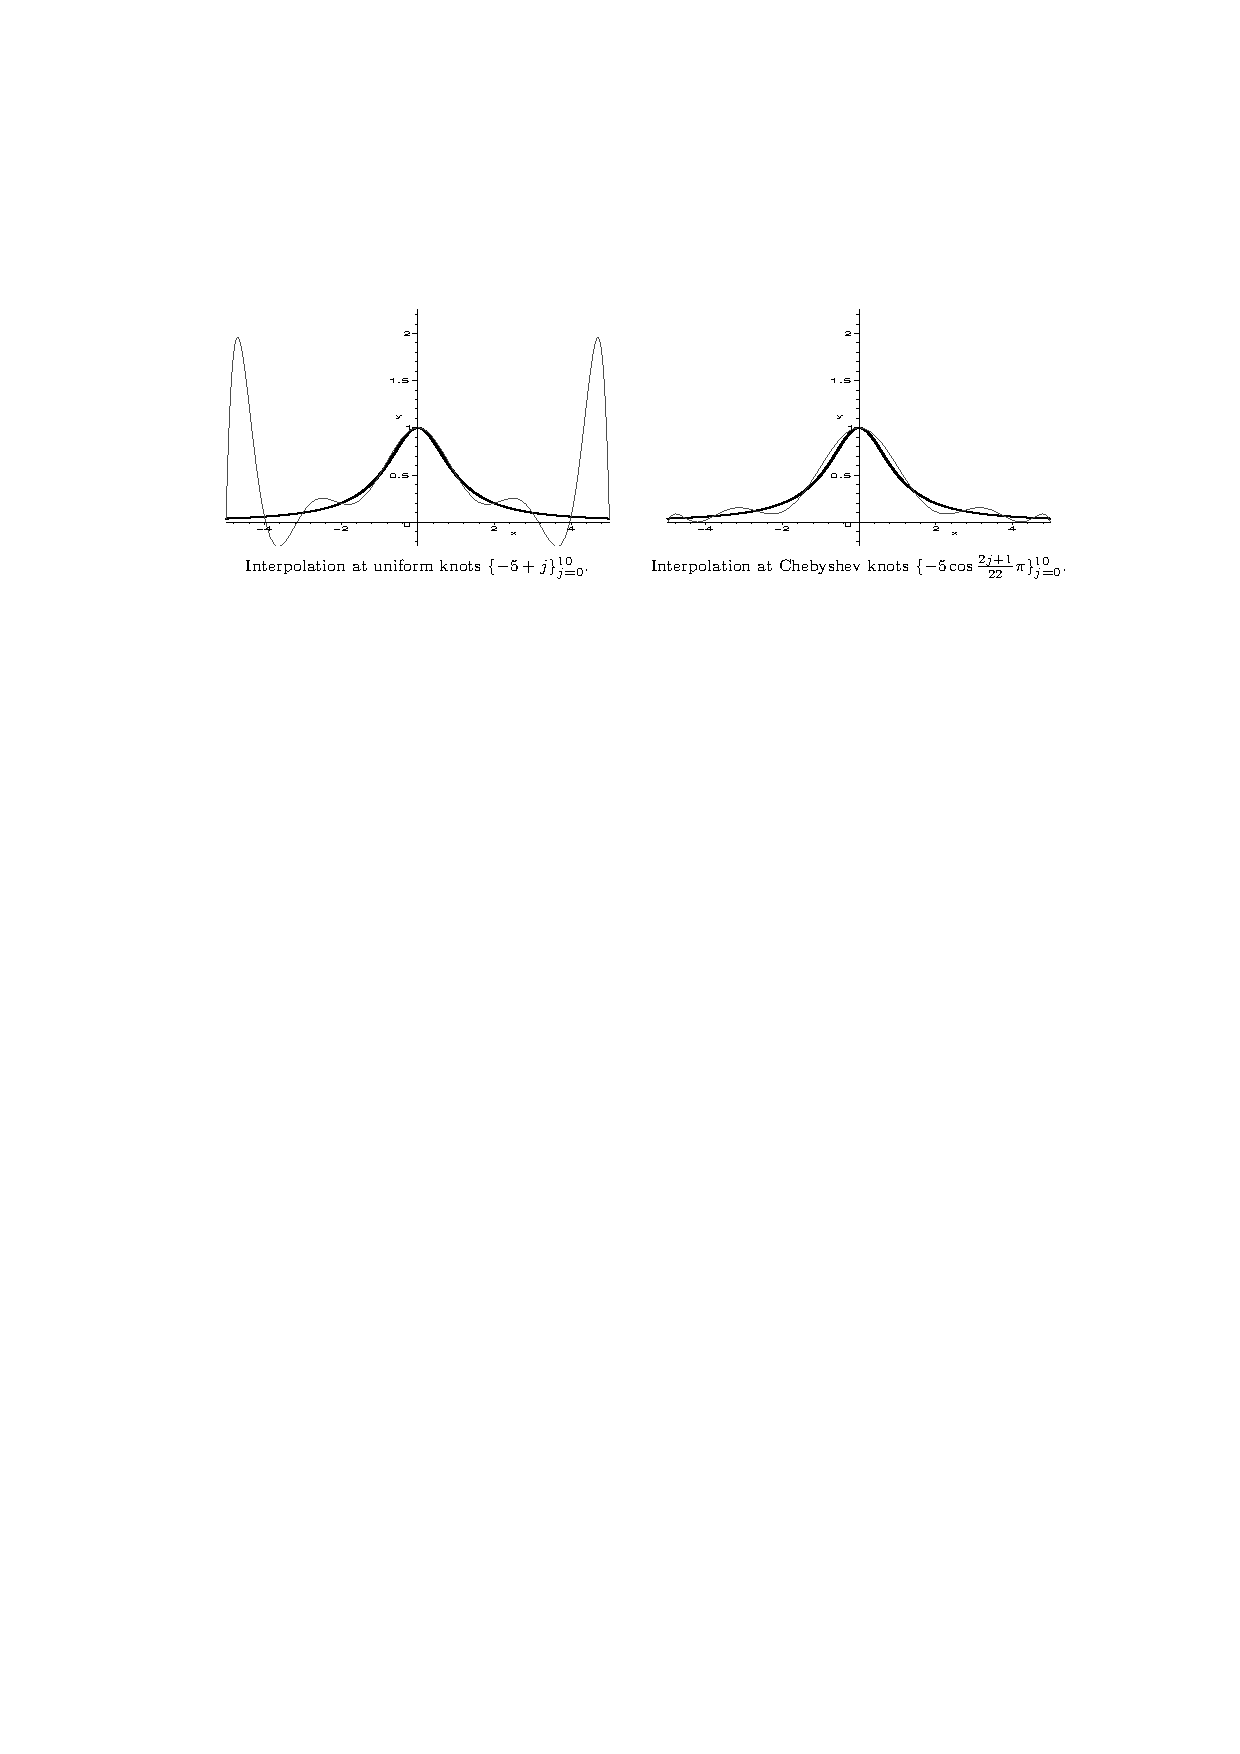
\includegraphics[scale=.85]{NA1}
    \end{center}
\end{example}

\begin{definition}
    The Chebyshev polynomial of degree $n$ on $[-1,1]$ is defined by
    \[
    T_n(x)=\cos n \theta, \quad x=\cos \theta, \quad \theta \in[0, \pi] .
    \]
    (Or just $T_n(x)=\cos (n \arccos x)$, with $x \in[-1,1]$.)
\end{definition}

One sees at once that, on $[-1,1]$,
\begin{enumerate}
    \item  $T_n$ takes its maximal absolute value 1 with alternating signs $n+1$ times:
    \[
    \left\|T_n\right\|_{\infty}=1, \quad T_n\left(t_k\right)=(-1)^k, \quad t_k=\cos \tfrac{\pi k}{n}, \quad k=\overline{0, n}
    \]
    \item $T_n$ has $n$ distinct zeros: $\quad T_n\left(x_k^*\right)=0, \quad x_k^*=\cos \frac{2 k-1}{2 n} \pi, \quad k=\overline{1, n}$.
\end{enumerate}

\begin{lemma}
    The Chebyshev polynomials $T_n$ satisfy the recurrence relation
    \begin{align}
        & T_0(x) \equiv 1, \quad T_1(x)=x, \label{eqn:2.4}\\
        & T_{n+1}(x)=2 x T_n(x)-T_{n-1}(x), \quad n \geq 1 .\label{eqn:2.5}
    \end{align}
    In particular, $T_n$ is an algebraic polynomial of degree $n$ with the leading coefficient $2^{n-1}$.
\end{lemma}
\begin{proof}
    Expressions (\ref{eqn:2.4}) are straightforward, the recurrence follows via the substitution $x=\cos \theta$ into identity $\cos (n+1) \theta+\cos (n-1) \theta=2 \cos \theta \cos n \theta$.
\end{proof}

\begin{theorem}
    On the interoal $[-1,1]$, among all polynomials of degree $n$ with the leading coefficient equal to one, the Chebyshev polynomial $\gamma T_n$ has the smallest max-norm, i.e.,
    \[
    \inf _{\left(a_i\right)}\left\|x^n+a_{n-1} x^{n-1}+\cdots+a_0\right\|_{\infty}=\left\|\gamma T_n\right\|_{\infty}=\gamma, \quad \gamma:=1 / 2^{n-1} .
    \]
\end{theorem}
\begin{proof}
    Suppose there is a polynomial $q_n(x)=x^n+a_{n-1} x^{n-1}+\cdots+a_0$ such that $\|q\|_{\infty}<\gamma$, and set
    \[
    r:=\gamma T_n-q_n .
    \]
    The leading coefficients of both $q_n$ and $\gamma T_n$ are equal 1 , thus $r$ is of degree at most $n-1$.

    Further, at $n+1$ points $t_k:=\cos \frac{\pi k}{n}$, the Chebyshev polynomial $\gamma T_n$ takes the values $\pm \gamma$ alternatively, while by assumption $\left|q_n\left(t_k\right)\right|<\gamma$, hence $r=\gamma T_n-q_n$ alternates in sign at these $n+1$ points, therefore it has a zero in each of $n$ intervals $\left(t_k, t_{k+1}\right)$, i.e. at least $n$ zeros in the interval $[-1,1]$, a contradiction to $r \in \mathcal{P}_{n-1}$.
\end{proof}

\begin{corollary}
    For $\Delta=\left(x_i\right)_{i=0}^n \subset[-1,1]$, let $\omega_{\Delta}(x)=\prod_{i=0}^n\left(x-x_i\right)$. Then, for all $n$, we have
    \[
    \inf _{\Delta}\left\|\omega_{\Delta}\right\|_{\infty}=\left\|\omega_{{\Delta}_{*}}\right\|_{\infty}=1 / 2^n .
    \]
\end{corollary}

\begin{theorem}
    For $f \in C^{n+1}[-1,1]$, the best choice of interpolating points is $\Delta_*=\left(x_i^*\right)=\left(\cos \frac{2 i+1}{2 n+2} \pi\right)_{i=0}^n$ and
    \[
    \left\|f-p_{\Delta_*}\right\|_{\infty} \leq \frac{1}{2^n} \frac{1}{(n+1) !}\left\|f^{(n+1)}\right\|_{\infty}
    \]
\end{theorem}

\begin{example}
    For $f(x)=e^x$, and $x \in[-1,1]$, the error of approximation provided by interpolating polynomial of degree 9 with 10 Chebyshev knots is bounded by
    \[
    \left|e^x-p_9(x)\right| \leq \frac{1}{2^9} \frac{1}{10 !} e \leq 1.5 \cdot 10^{-9}
    \]
\end{example}

\section{Orthogonal polynomials}
\subsection{The three-term recurrence relation}
Consider $\mathbb{X}=C[a, b]$, the space of all continuous real-valued functions $f:[a, b] \rightarrow \mathbb{R}$, and define a \textbf{scalar} (or \textbf{inner}) \textbf{product} on $C[a, b]$ by
\begin{equation}\label{eqn:3.1}
    (f, g):=(f, g)_w:=\int_a^b f(x) g(x) w(x) d x .
\end{equation}
Here $w$, the so-called \textbf{weight function}, is a fixed positive function, such that the integral $\int h(x) w(x) d x$ exists for all $h \in C[a, b]$.

We denote by $\mathcal{P}_n$ the space of all algebraic polynomials of degree (at most) $n$, i.e., $p \in \mathcal{P}_n$ if $p(x)=\sum_{k=0}^n a_k x^k$. If the leading coefficent $a_n$ equals 1 , then $p$ is called a \textbf{monic} polynomial. Given a scalar product (\ref{eqn:3.1}), we say that $Q_n \in \mathcal{P}_n$ is the $n$\textbf{-th} \textbf{orthogonal polynomial} if
\[
\left(Q_n, p\right)=0 \quad \forall p \in \mathcal{P}_{n-1} .
\]
Different weights lead to different orthogonal polynomials.

\begin{lemma}
    For every $n \in \mathbb{N}$, there exists a unique monic orthogonal polynomial $Q_n \in \mathcal{P}_n$. Any $p \in \mathcal{P}_n$ is uniquely expressible as a linear combination
    \begin{equation}\label{eqn:3.2}
        p=\sum_{k=0}^n c_k Q_k, \quad c_k=\left(p, Q_k\right) /\left\|Q_k\right\|^2
    \end{equation}
\end{lemma}
\begin{proof}
    We apply the Gram-Schmidt orthogonalization algorithm for the linearly independent sequence of monomials $\left(1, x, \ldots, x^n, \ldots\right)$. Starting with $Q_0 \equiv 1$ we set
\[
Q_n(x):=x^n-\sum_{k=0}^{n-1} \frac{\left(x^n, Q_k\right)}{\left(Q_k, Q_k\right)} Q_k(x), \quad n=1,2, \ldots
\]
Then, from construction, $\left(Q_n, Q_k\right)=0$, i.e., $Q_n$ is orthogonal to each previous $Q_k$. Also, we have $x^n \in \operatorname{span}\left(Q_k\right)_{k=0}^n$, hence $\mathcal{P}_n=\operatorname{span}\left(Q_k\right)_{k=0}^n$. Therefore $Q_n \perp \mathcal{P}_{n-1}$, and any $p \in \mathcal{P}_n$ has an expansion (\ref{eqn:3.2}). Each coefficient $c_k$ in (\ref{eqn:3.2}) is uniquely determined by multiplying both sides (in the scalar product sense) with $Q_k$.

If $\widetilde{Q}_n$ is another $n$-th monic orthogonal polynomial, then $p:=Q_n-\widetilde{Q}_n$ belongs to $\mathcal{P}_{n-1}$, therefore $(p, p)=\left(Q_n-\widetilde{Q}_n, p\right)=0$. Hence $p \equiv 0$ (by the scalar product property), i.e., $\widetilde{Q}_n \equiv Q_n$.
\end{proof}
\begin{remark}
    For practical construction of orthogonal polynomials the Gram-Schmidt is not of much help, for it leads to loss of accuracy due to imprecisions in calculation of scalar products. A considerably better procedure is being provided by the next theorem.
\end{remark}

\begin{theorem}[The three-term recurrence relation]
    Monic orthogonal polynomials satisfy the relation
    \begin{equation}\label{eqn:3.3}
        Q_{n+1}(x)=\left(x-a_n\right) Q_n(x)-b_n Q_{n-1}(x), \quad n=0,1, \ldots
    \end{equation}
    where $Q_{-1}(x) \equiv 0, Q_0(x) \equiv 1$, and
    \begin{equation}\label{eqn:3.4}
        a_n=\frac{\left(x Q_n, Q_n\right)}{\left(Q_n, Q_n\right)}, \quad b_n=\frac{\left(Q_n, Q_n\right)}{\left(Q_{n-1}, Q_{n-1}\right)}>0
    \end{equation}
\end{theorem}
\begin{proof}
    Based on (\ref{eqn:3.2}), let us look at the coefficients of the expansion
    \[
    x Q_n(x)=\sum_{k=0}^{n+1} c_k Q_k(x), \quad c_k=\frac{\left(x Q_n, Q_k\right)}{\left(Q_k, Q_k\right)}=\frac{\left(Q_n, x Q_k\right)}{\left(Q_k, Q_k\right)},
    \]
    using the last (equivalent) formula for $c_k$.

    $k=n+1 \to  c_{n+1}=1$, since both $x Q_n(x)$ and $Q_{n+1}(x)$ are monic polynomials of degree $n+1$.

    $k=n \to  c_n=a_n$ in (\ref{eqn:3.4}).

    $k=n-1 \to $ Because of monicity, we have the equality $x Q_{n-1}=Q_n+p_{n-1}$ where $p_{n-1} \in \mathcal{P}_{n-1}$, so that $\left(Q_n, x Q_{n-1}\right)=\left(Q_n, Q_n+p_{n-1}\right)=\left(Q_n, Q_n\right)$, hence $c_{n-1}=b_n$ in (\ref{eqn:3.4}).

    $k<n-1 \to $ Then $x Q_k \in \mathcal{P}_{n-1}$, and we obtain $\left(Q_n, x Q_k\right)=0$, thus $c_k=0$.

    It follows that $x Q_n(x)=Q_{n+1}+a_n Q_n+b_n Q_{n-1}$, and that is equivalent to (\ref{eqn:3.3})-(\ref{eqn:3.4})
\end{proof}
\begin{remark}
    If $\left(Q_k\right)$ have leading coefficients $\left(\alpha_k\right)$, then the recurrence takes the form
    \[
    Q_{n+1}(x)=\frac{\alpha_{n+1}}{\alpha_n}\left(x-a_n\right) Q_n(x)-\frac{\alpha_{n+1} \alpha_{n-1}}{\alpha_n^2} b_n Q_{n-1}(x), \quad n=0,1, \ldots
    \]
    and, with an appropriate choice of $\left(\alpha_k\right)$, may become very simple.
\end{remark}

\subsection{Examples}
\ \vspace*{-1.5em}

\begin{example}
    Classical examples of orthogonal (non-monic) polynomials include
    \begin{center}
        \begin{tabular}{lcccc}
            \toprule 
            \bfseries Name &\bfseries {Notation} &\bfseries {Interval} & \bfseries{Weight} &\bfseries {Recurrence} \\
            \midrule {Legendre} & $P_n$ & ${[-1,1]}$ &  $1$ & $(n+1) P_{n+1}(x)=(2 n+1) x P_n(x)-n P_{n-1}(x)$ \\[.6em]
            {Chebyshev} & $T_n$ & ${[-1,1]}$ & $\left(1-x^2\right)^{-1 / 2}$ & $T_{n+1}(x)=2 x T_n(x)-T_{n-1}(x)$ \\[.6em]
            {Laguerre} & $L_n$ & ${[0, \infty)}$ & ${e}^{-x}$ & $(n+1) L_{n+1}(x)=(2 n+1-x) L_n(x)-n L_{n-1}(x)$ \\[.6em]
            {Hermite} & $H_n$ & $(-\infty, \infty)$ & ${e}^{-x^2}$ & $H_{n+1}(x)=2 x H_n(x)-2 n H_{n-1}(x)$ \\
            \bottomrule
        \end{tabular}
    \end{center}
\end{example}

\begin{example}[The Chebyshev polynomials]
    The Chebyshev polynomials $T_n$, on line 2 in the table above, were introduced in Lecture 2 as
    \[
    T_n(x)=\cos n \arccos x, \quad x \in[-1,1],
    \]
    where we also proved the three-term recurrence relation. Let us show that they are indeed orthogonal with the weight $w(x)=\left(1-x^2\right)^{-1 / 2}$. With the substistuion $x=\cos \theta, \theta \in[0, \pi]$ we have $T_n(x)=\cos n \theta$ and
    \[
    \begin{aligned}
    \left(T_n, T_m\right)_w & :=\int_{-1}^1 T_n(x) T_m(x) \frac{\dd x}{\sqrt{1-x^2}}\\ 
    &=\int_0^\pi \cos n \theta \cos m \theta \dd \theta=\frac{1}{2} \int_{-\pi}^\pi \cos n \theta \cos m \theta \dd \theta \\
    & =\frac{1}{4} \int_{-\pi}^\pi[\cos (n+m) \theta+\cos (n-m) \theta] \dd \theta=0, \quad n \neq m .
    \end{aligned}
    \]
\end{example}

\subsection{Least squares polynomial fitting}
Let $f$ be a continuous function defined on some interval $[a, b]$, and suppose we wish to approximate $f$ by a polynomial of degree $n$. If we equip $C[a, b]$ with the distance $\|f-g\|:=(f-g, f-g)^{1 / 2}$ induced by a scalar product $(f, g)=f_a^b f(x) g(x) w(x) d x$, then it is natural to seek a polynomial
\[
p^*:=\arg \min _{p \in \mathcal{P}_n}\|f-p\|,
\]
for which the distance $\left\|f-p^*\right\|$ is as small as possible. Such a polynomial is called a (weighted) \textbf{least squares approximant}.

\begin{theorem}
    Let $\left(Q_k\right)_{k=0}^n$ be polynomials orthogonal with respect to a given inner product. Then the least squares approximant to any $f \in C[a, b]$ from $\mathcal{P}_n$ is given by the formula
    \begin{equation}\label{eqn:3.5}
        p^*=p^*(f)=\sum_{k=0}^n c_k^* Q_k, \quad c_k^*=\frac{\left(f, Q_k\right)}{\left\|Q_k\right\|^2},
    \end{equation}
    and the value of the least squares approximation is
    \begin{equation}\label{eqn:3.6}
        \left\|f-p^*\right\|^2=\|f\|^2-\sum_{k=1}^n \frac{\left(f, Q_k\right)^2}{\left\|Q_k\right\|^2} .
    \end{equation}
\end{theorem}
\begin{remark}
    By orthogonality of $Q_k$, the norm of the extremal $p^*$ is equal to
    \[
    \left\|p^*\right\|^2=\left\|\sum_{k=0}^n c_k^* Q_k\right\|^2=\sum_{k=0}^n\left|c_k^*\right|^2\left\|Q_k\right\|^2=\sum_{k=1}^n \frac{\left(f, Q_k\right)^2}{\left\|Q_k\right\|^2},
    \]
    hence formula (3.6) takes the form
    \[
    \left\|f-p^*\right\|^2=\|f\|^2-\left\|p^*\right\|^2,
    \]
    which is a reminiscent of the Pythagoras theorem.
\end{remark}
\begin{proof}
    Let $p=\sum_{k=0}^n c_k Q_k$. Then
    \begin{align}\label{eqn:3.7}
        F(c)&=(f-p, f-p)=\left(f-\sum_{k=0}^n c_k Q_k, f-\sum_{k=0}^n c_k Q_k\right)\nonumber \\ 
        &=\|f\|^2-2 \sum_{k=0}^n c_k\left(f, Q_k\right)+\sum_{k=0}^n c_k^2\left\|Q_k\right\|^2
    \end{align}
    The right-hand side is a quadratic polynomial in each $c_k$, therefore it attains its minimum when
    \[
    \eval{\frac{\partial F}{\partial c_k}}_{c_k=c_k^*}=-2\left(f, Q_k\right)+2 c_k^*\left\|Q_k\right\|^2=0, \quad k=\overline{0, n},
    \]
    hence conclusion (\ref{eqn:3.5}). Putting optimal $c_k^*$ into (\ref{eqn:3.7}) we obtain (\ref{eqn:3.6}).
\end{proof}

\begin{method}
    Suppose we want to approximate $f \in C[a, b]$ with a prescribed accuracy $\epsilon$, i.e., to find $n=n(\epsilon)$ such that
    \[
    \left\|f-p^*\right\| \leq \epsilon, \quad p^* \in \mathcal{P}_n .
    \]
    From (\ref{eqn:3.6}), it follows that the required value $n$ can be calculated by summing the terms of $\frac{\left(f, Q_k\right)^2}{\left\|Q_k\right\|^2}$ until we reach the bound
    \[
    \sum_{k=1}^n \frac{\left(f, Q_k\right)^2}{\left\|Q_k\right\|^2} \geq\|f\|^2-\epsilon^2 .
    \]
\end{method}

The next theorem assures that this bound can be reached.

\begin{theorem}[The Parseval identity]
    If $[a, b]$ is finite, then $ \displaystyle \sum_{k=0}^{\infty} \frac{\left(f, Q_k\right)^2}{\left\|Q_k\right\|^2}=\|f\|^2$.
\end{theorem}
\begin{proof}[Proof (incomplete)]
    Let
    \[
    \sigma_n^2:=\left\|p^*\right\|^2=\sum_{k=0}^n \frac{\left(f, Q_k\right)^2}{\left\|Q_k\right\|^2},
    \]
    hence
    \[
    \inf_{p \in \mathcal{P}_n}\|f-p\|^2=\left\|f-p^*\right\|^2=\|f\|^2-\sigma_n^2 .
    \]
    According to the Weierstrass theorem, any function in $C[a, b]$ can be approximated arbitrarily close by a polynomial, hence $\lim _{n \rightarrow \infty} \inf _{p \in \mathcal{P}_n}\|f-p\|^2=0$ and we deduce that $\sigma_n^2 \rightarrow\|f\|^2$ as $n \rightarrow \infty$.
\end{proof}
\end{document}